% 2009 年广东卷（文科）第 15 题：圆 O 上三点 A、B、C，AB=4，∠ACB=30°。
% 来源 PDF：.work/ocr-local/sources/2009广东文.pdf
% SHA-256：26c26718ce8f1cd1128fca4e63e1576ecec72ee27cc46ad538673bb533e61ced
% 原页：第 1 页（A3 三栏）第 3 栏，印刷页 521。
% 绘制依据：B 在 60°、A 在 0°、C 在 240°，AB 为右侧弦，C 在下方；
%   圆周角 ∠ACB=30° 对应 AB 所对圆心角 60°。
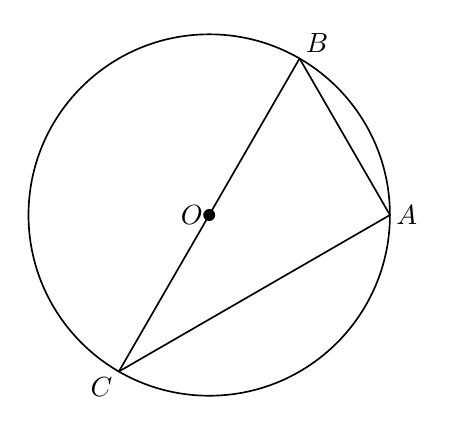
\begin{tikzpicture}[scale=1.35, semithick, every node/.style={inner sep=2pt}]
  \draw (0,0) circle (1.7);
  \coordinate (O) at (0,0);
  \coordinate (B) at (60:1.7);
  \coordinate (A) at (0:1.7);
  \coordinate (C) at (240:1.7);

  \draw (A) -- (B);
  \draw (C) -- (B);
  \draw (C) -- (A);

  \fill (O) circle (1.6pt);
  \node[left] at (0,0) {$O$};
  \node[above right] at (B) {$B$};
  \node[right] at (A) {$A$};
  \node[below left] at (C) {$C$};
\end{tikzpicture}
